% team-meeting-2026-11-09-slides.tex -- summary slides on the multi-model results for
% the team meeting of November 9, 2026.
% Build: plain pdflatex (emacs, emacs-r container) or xelatex (bittensor-ubuntu), run
% twice. beamerthemeozlabs.sty, ozcolors.sty and ozfonts.sty in this directory are
% symlinks to ~/code/oz-templates/, and the logo is set by absolute path below, so no
% TEXINPUTS setting is needed.
% Numbers come from docs/reports/multimodel-2026-11/ (tables/, tex-tables/,
% multimodel-summary.tex); figures are made by output/report-multimodel-2026-11/make_figures.R.
\documentclass[aspectratio=169,11pt]{beamer}

\usetheme{ozlabs}

\renewcommand{\ozfootbrand}{OZ Labs}
\renewcommand{\ozfooturl}{ozlabs.tech}
\renewcommand{\ozeyelogo}{/var/home/aoz/code/oz-templates/assets/ozlabs-seed-logo.pdf}

\usepackage{booktabs}
\usepackage{array}
\newcolumntype{L}[1]{>{\raggedright\arraybackslash}p{#1}}

\title{Heat and Cold Deaths, 2022--2050: Multi-Model Results}
\subtitle{204 countries, four climate scenarios, 24 climate models, with uncertainty ranges}
\author{Aaron Osgood-Zimmerman}
\institute{OZ Labs, for the World Bank}
\date{November 9, 2026}

\begin{document}

\begin{frame}[plain,noframenumbering]
  \titlepage
\end{frame}

\begin{frame}{Where we are}
  \begin{itemize}
    \item Caspar's per-draw run has arrived and passes my checks; nothing more is needed from him for these results. Thanks, Caspar!
    \item Everything here follows what we agreed on October 27: the 24 models run under all four scenarios, keeping the adjustment to IHME's forecasts, heat and cold side by side, decade averages.
    \item SSP2-4.5 is the reference scenario: IHME's mortality forecast is defined under it, and the other three are compared against it. Every figure shows it.
    \item Each number pools 24 models $\times$ 500 draws = 12,000 values, so its range includes disagreement between climate models. Ranges are 95\%, 80\% and 66\%; the figures show all three (thin, medium, thick bars).
    \item A draft report with all the tables goes with these slides. Today: the main results, my cautions, and a few questions for the team.
  \end{itemize}
\end{frame}

\begin{frame}{World: heat and cold both rise in every scenario}
  \centering
  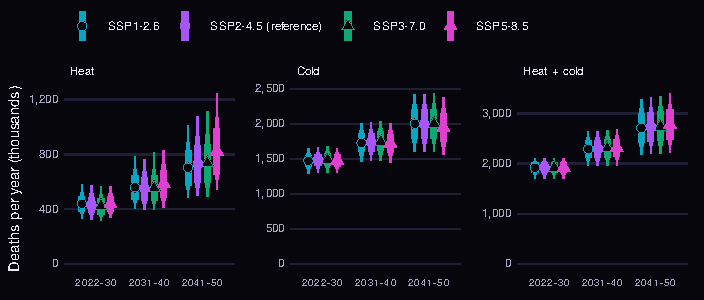
\includegraphics[width=0.84\textwidth]{figures-2026-11-09/fig_world_decades.pdf}

  \small\raggedright
  Under SSP2-4.5 (the reference), from 2022--2030 to 2041--2050: heat 431,244 to 729,507 deaths per year, cold 1,483,673 to 1,998,935. Cold stays the larger burden; heat's share of the two goes from 22.5\% to 26.7\%.
\end{frame}

\begin{frame}{Cold deaths rise because deaths from these causes rise}
  \centering
  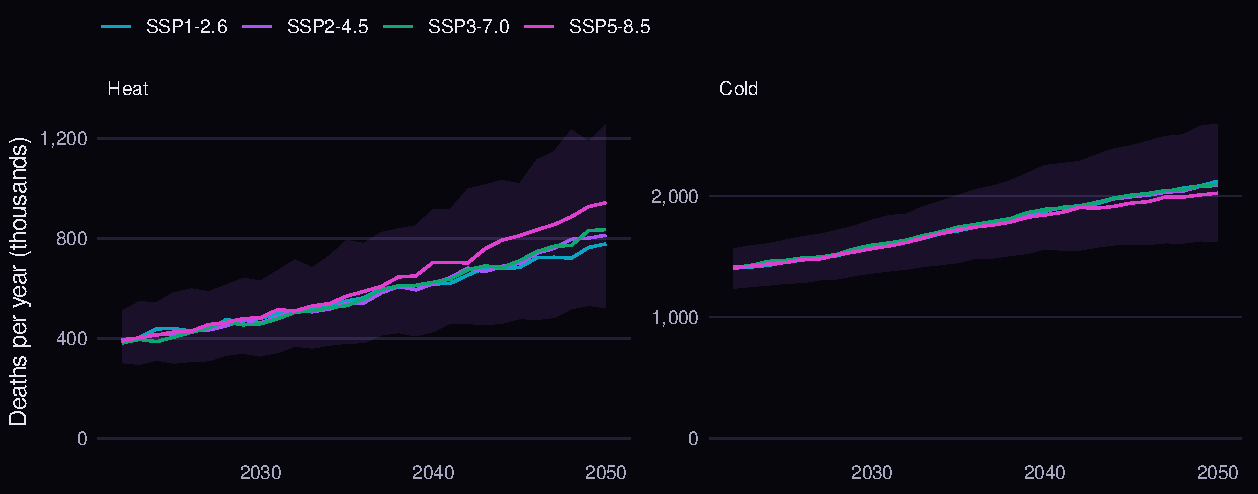
\includegraphics[width=0.62\textwidth]{figures-2026-11-09/fig_world_yearly.pdf}

  \footnotesize\raggedright
  \begin{itemize}
    \item Under SSP2-4.5, IHME's forecast of deaths from these 17 causes grows from 32.0 to 43.4 million per year (+36\%) between 2022--2030 and 2041--2050, most likely from population growth and aging (not split here).
    \item Cold's share of those deaths stays flat (4.66\% to 4.62\%), so cold deaths grow with them even though it gets warmer. Heat's share rises (1.32\% to 1.69\%), so heat grows faster.
    \item Single years are noisy (the band is the SSP2-4.5 95\% range), which is why we report decades.
  \end{itemize}
\end{frame}

\begin{frame}{Scenarios differ more in the split than in the total}
  \centering
  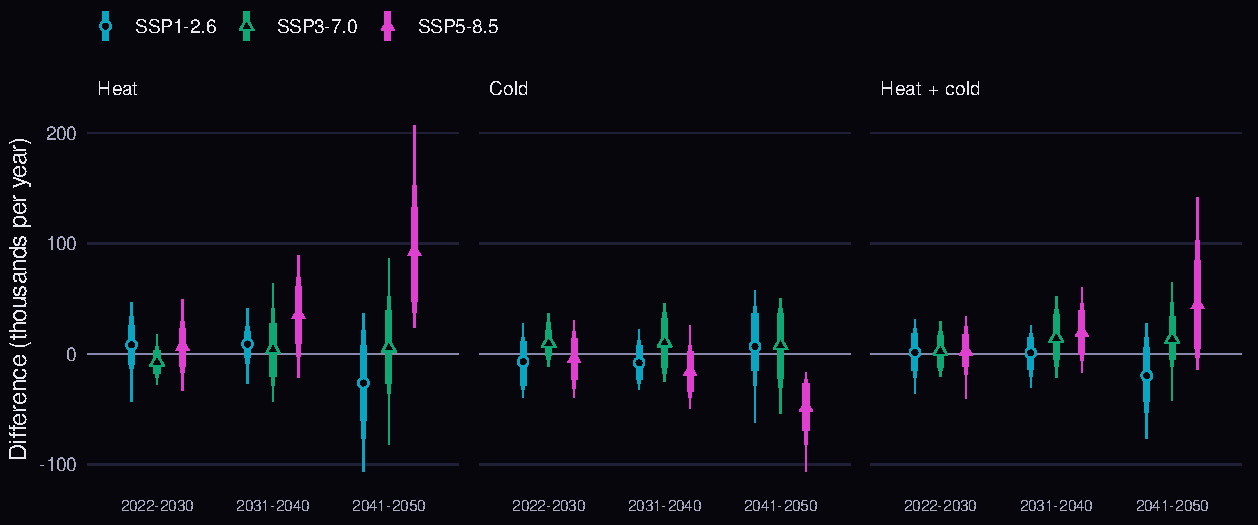
\includegraphics[width=0.84\textwidth]{figures-2026-11-09/fig_world_diff.pdf}

  \small\raggedright
  Differences from SSP2-4.5, taken draw by draw within each climate model; SSP2-4.5 is zero by definition (its levels are on the earlier world slide). A warmer scenario adds heat deaths and removes cold deaths, so the total barely moves.
\end{frame}

\begin{frame}{Scenarios against SSP2-4.5 (reference), world, 2041--2050}
  \scriptsize
  \centering
  \renewcommand{\arraystretch}{0.84}\setlength{\tabcolsep}{5pt}
  \begin{tabular}{llcccc}
    \toprule
    & & Deaths per year & Change from & Difference & Models with \\
    & & (thousands, 95\% range) & SSP2-4.5 & (thousands, 95\% range) & more deaths \\
    \midrule
    Heat & SSP1-2.6 & 703 (482 to 1,014) & $-3.6$\% & $-26$ ($-107$ to 37) & 7 of 24 \\
         & SSP2-4.5 & 730 (499 to 1,074) & reference & & \\
         & SSP3-7.0 & 735 (495 to 1,116) & $+0.8$\% & 6 ($-82$ to 86) & 13 of 24 \\
         & SSP5-8.5 & 822 (543 to 1,244) & $+12.7$\% & 92 (24 to 207) & 24 of 24 \\
    \midrule
    Cold & SSP1-2.6 & 2,006 (1,610 to 2,429) & $+0.3$\% & 7 ($-62$ to 57) & 13 of 24 \\
         & SSP2-4.5 & 1,999 (1,603 to 2,424) & reference & & \\
         & SSP3-7.0 & 2,007 (1,608 to 2,436) & $+0.4$\% & 8 ($-54$ to 50) & 16 of 24 \\
         & SSP5-8.5 & 1,951 (1,560 to 2,374) & $-2.4$\% & $-48$ ($-107$ to $-17$) & 0 of 24 \\
    \midrule
    Heat + cold & SSP1-2.6 & 2,709 (2,185 to 3,286) & $-0.7$\% & $-20$ ($-77$ to 28) & 5 of 24 \\
         & SSP2-4.5 & 2,728 (2,198 to 3,316) & reference & & \\
         & SSP3-7.0 & 2,742 (2,209 to 3,337) & $+0.5$\% & 14 ($-42$ to 65) & 19 of 24 \\
         & SSP5-8.5 & 2,773 (2,225 to 3,395) & $+1.6$\% & 44 ($-14$ to 141) & 21 of 24 \\
    \bottomrule
  \end{tabular}

  \smallskip
  \raggedright\scriptsize
  \emph{Change}: scenario mean over its 12,000 values $\div$ SSP2-4.5 mean, minus 1. \emph{Difference}: scenario minus SSP2-4.5 within each climate model and draw, then pooled, so uncertainty shared by both scenarios cancels. \emph{Climate models with more deaths}: how many of the 24 models have a higher average under the scenario than under SSP2-4.5; about 12 means no agreement on direction, and the models share code, so 24 of 24 is not 24 independent results.
  The range of the difference excludes zero only for SSP5-8.5 heat and cold, and for no total.
\end{frame}

\begin{frame}{Climate model choice matters for heat, hardly for the total}
  \small
  Share of the variance of the 12,000 pooled values (24 models $\times$ 500 draws) that is between climate models, i.e.\ the variance of the 24 model averages; world, 2041--2050:

  \medskip
  \centering
  \begin{tabular}{lcccc}
    \toprule
    & SSP1-2.6 & SSP2-4.5 & SSP3-7.0 & SSP5-8.5 \\
    \midrule
    Heat deaths & 41\% & 44\% & 50\% & 49\% \\
    Cold deaths & 7\% & 8\% & 9\% & 10\% \\
    Heat + cold & 2\% & 3\% & 3\% & 4\% \\
    \bottomrule
  \end{tabular}

  \medskip
  \raggedright\footnotesize
  \begin{itemize}
    \item The rest (for heat + cold, 96 to 98\%) is within models, across the 500 draws. A draw is one draw of the 17 risk curves (and the minimum-risk temperature derived from them) with one draw of IHME's mortality forecast; this run can't separate the two.
    \item The point: about half the range on heat comes from which climate model is used, but almost none of the range on the total, because a model that runs warm has more heat and less cold. The range on the total reflects the risk curves and the mortality forecast.
    \item Not in any range: the bias correction of temperature, the choice of curves, and the fact that our 24 models aren't independent.
  \end{itemize}
\end{frame}

\begin{frame}{Income groups: the burden differs in kind}
  \centering
  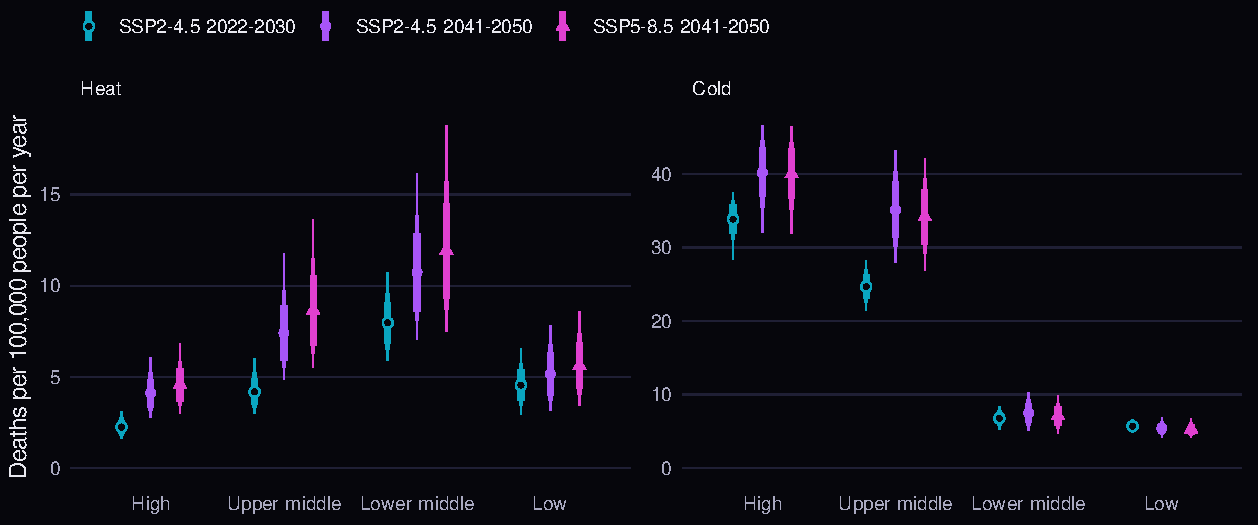
\includegraphics[width=0.9\textwidth]{figures-2026-11-09/fig_income_rates.pdf}

  \footnotesize\raggedright
  One column per decade, all four scenarios in each. Crude rates, not age-standardized, so much of the cold contrast is likely age structure. Low- and middle-income countries hold 92\% of heat deaths and 71\% of cold deaths in 2041--2050, in every scenario. World Bank groups held fixed at today's classification; the mapping still needs a second look.
\end{frame}

\begin{frame}{Countries: rates under SSP2-4.5 (reference), 2041--2050}
  \centering
  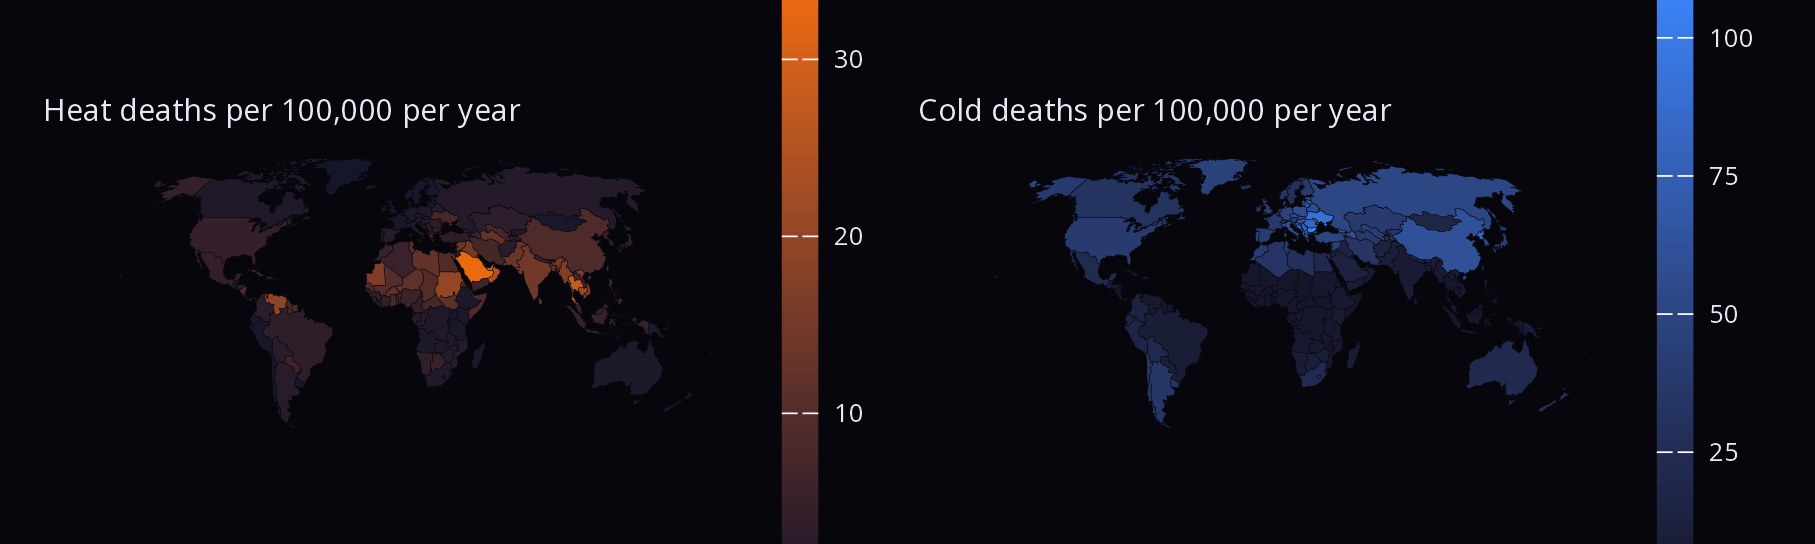
\includegraphics[width=\textwidth]{figures-2026-11-09/fig_maps.png}

  \small\raggedright
  \begin{itemize}
    \item The totals are concentrated: India has 31.7\% of heat deaths, China 39.6\% of cold deaths.
    \item Caution on the Gulf. IHME has 17-cause deaths in the UAE growing by 10.6 times from 2022 to 2050 (world: 1.52), with the population aged 65+ going from 198,137 to 4,717,387. My guess is migrant workers forecast to age in place. It puts Saudi Arabia (33.4 per 100,000) and the UAE (29.2) at the top of the heat rate table.
  \end{itemize}
\end{frame}

\begin{frame}{Causes, world, 2041--2050, all four scenarios}
  \begin{columns}[T,onlytextwidth]
  \begin{column}{0.6\textwidth}
  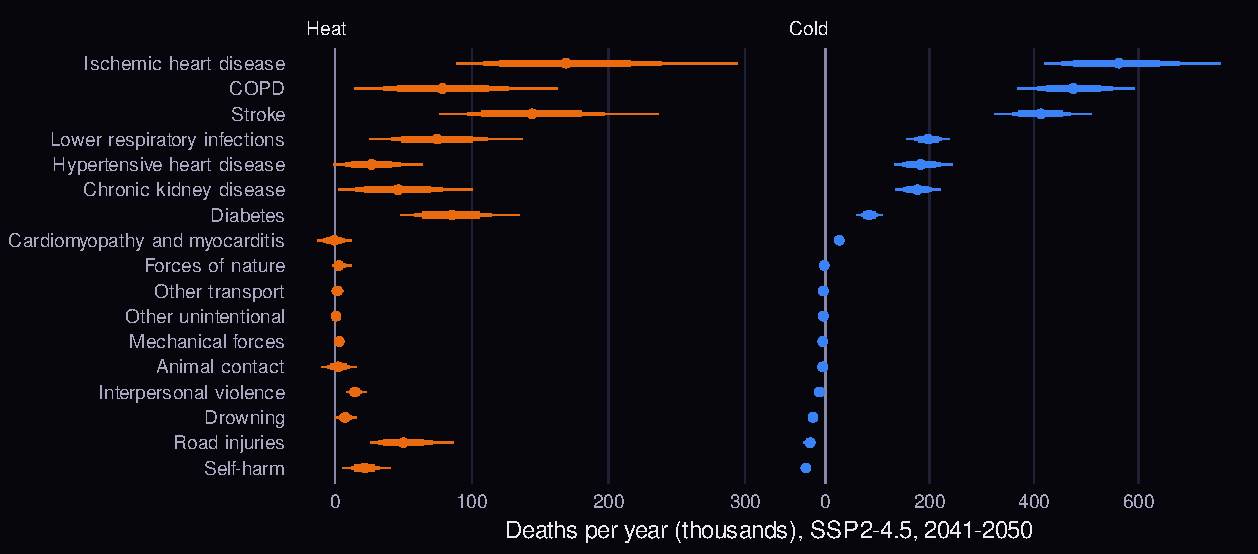
\includegraphics[width=\textwidth]{figures-2026-11-09/fig_causes.pdf}
  \end{column}
  \begin{column}{0.38\textwidth}
  \scriptsize\raggedright
  \begin{itemize}
    \item Every cause has heat and cold deaths: days above the country's minimum-risk temperature count toward heat, days below toward cold.
    \item Negative cold: fewer deaths on cold days than at the minimum-risk temperature. That temperature is set by all 17 causes together, weighted by their deaths, not by injuries alone, and injury risk is lower on colder days than at it. The nine injury causes sum to $-118{,}826$ per year (SSP2-4.5), kept in the cold total.
    \item The four scenarios overlap for every cause.
  \end{itemize}
  \end{column}
  \end{columns}
\end{frame}

\begin{frame}{Narrow cells: the range often includes zero}
  \begin{itemize}
    \item When the 95\% range includes zero, the data can't tell whether temperature adds or removes deaths in that cell. The mean is still our best estimate, but its sign isn't established, so it shouldn't be read as a finding on its own. Nothing is wrong with the numbers.
    \item This is common for single causes. World level: the range includes zero for 7 of 17 causes for heat and 1 of 17 for cold (SSP2-4.5, 2041--2050).
    \item One cause in one country: it includes zero in 60\% of cells for heat and 29\% for cold (SSP2-4.5, 2041--2050; 60\% and 29 to 31\% across the four scenarios).
    \item Country totals rarely do: in any scenario and decade, at most 2 of 204 countries for heat, 2 for cold, and none for heat + cold.
    \item So the draft report shows causes at world and income-group level, and country by cause only in an appendix, with those cells in parentheses.
  \end{itemize}
\end{frame}

\begin{frame}{Age and sex, world}
  \centering
  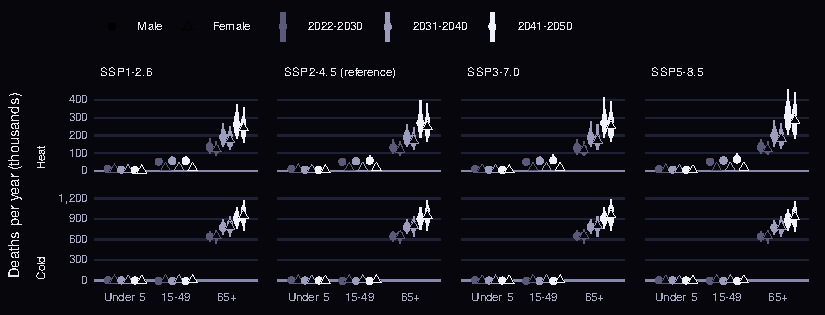
\includegraphics[width=0.92\textwidth]{figures-2026-11-09/fig_age.pdf}

  \scriptsize\raggedright
  \begin{itemize}
    \item Color is the decade (darker to lighter), symbol is sex. The four scenarios look alike. Under SSP2-4.5, 65+ goes from 59\% to 72\% of heat deaths, and from 88\% to 93\% of cold deaths. Under-5 heat deaths halve (21,009 to 10,766 per year) as under-5 mortality falls in the forecast.
    \item Men aged 15--49 have about three times the heat deaths of women, and a slightly negative cold total. I suspect injuries in both cases, not yet split.
  \end{itemize}
\end{frame}

\begin{frame}{Years of life lost: one thing to be careful about}
  \begin{itemize}
    \item Under SSP2-4.5 in 2041--2050: heat 12.8 million years per year (8.7 to 18.9 million), cold 23.8 million (18.9 to 29.4 million). These use each country's own life table, so they aren't comparable with GBD's.
    \item A country's cold years of life lost can be negative alongside positive cold deaths. Injuries have negative cold values (the country's minimum-risk temperature is set by all 17 causes together, and for injuries cold days carry less risk than that temperature), and injury deaths happen at young ages, so each one carries many years of life.
    \item This holds for 21 countries in 2022--2030, 13 in 2031--2040 and 8 in 2041--2050. For example, Burkina Faso (SSP1-2.6, 2041--2050): +114.6 cold deaths, $-294.9$ years.
    \item \textbf{My suggestion:} report it as it is, with a note, and don't publish years of life lost per death wherever signs mix.
  \end{itemize}
\end{frame}

\begin{frame}{Haiti and Honduras: the asterisk}
  \small
  Heat + cold deaths per year, SSP2-4.5:

  \medskip
  \centering
  \begin{tabular}{llcc}
    \toprule
    & & All 17 causes (95\% range) & Without forces of nature (95\% range) \\
    \midrule
    Haiti$^{*}$    & 2022--2030 & 2,084 (282 to 10,715) & 236 ($-713$ to 603) \\
                   & 2041--2050 & 2,032 (417 to 8,575)  & 497 ($-461$ to 1,093) \\
    Honduras$^{*}$ & 2022--2030 & 547 (360 to 954)      & 407 (145 to 594) \\
                   & 2041--2050 & 818 (530 to 1,216)    & 702 (349 to 1,051) \\
    \bottomrule
  \end{tabular}

  \medskip
  \raggedright
  \begin{itemize}
    \item A few of IHME's forecast draws carry event-scale disaster deaths. All 17 causes stay in the headline, as we decided; these two get an asterisk and the second column.
    \item The second column is not a correction: in Haiti those draws also distort the minimum-risk temperature for every cause.
    \item Only these two move by more than 10\%; the world total moves by under 0.04\% (2041--2050). Single draws in Puerto Rico and Myanmar show it too.
  \end{itemize}
\end{frame}

\begin{frame}{The year heat overtakes cold}
  \small
  Samuel's question. For each country, a straight line through yearly heat minus cold deaths, fitted separately for each of the 12,000 (model, draw) pairs, gives 12,000 crossing years. The table counts countries (of 204) by where the median of those 12,000 years falls:

  \medskip
  \centering
  \begin{tabular}{lcccc}
    \toprule
    Number of countries & SSP1-2.6 & SSP2-4.5 & SSP3-7.0 & SSP5-8.5 \\
    \midrule
    Before 2022 (heat already above cold) & 83 & 82 & 80 & 75 \\
    Between 2022 and 2050   & 6  & 8  & 11 & 16 \\
    After 2050 (heat still below cold)    & 115 & 114 & 113 & 113 \\
    \bottomrule
  \end{tabular}

  \medskip
  \raggedright\footnotesize
  \begin{itemize}
    \item Where the median falls inside the period, the year can't be pinned down: under SSP2-4.5 there are eight such countries (for example Iraq, Dominican Republic, Honduras), and for all eight the 95\% range runs from before 2022 to after 2050.
    \item \textbf{My suggestion:} report, per country, the share of the 12,000 pairs in each of the three groups, not a year. Under SSP2-4.5: India 85\% before 2022, 15\% between, 0.3\% after; Iraq 33\%, 36\%, 32\%; China 0\%, 0\%, 100\%.
  \end{itemize}
\end{frame}

\begin{frame}{Model choice moves these comparisons by at most 1 point}
  \footnotesize
  Change from SSP2-4.5, world, 2041--2050, under three ways of choosing the climate models:

  \smallskip
  \centering
  \scriptsize\renewcommand{\arraystretch}{0.8}
  \begin{tabular}{llccc}
    \toprule
    & & Common 24 & Paired & All available \\
    \midrule
    Heat & SSP1-2.6 & $-3.6$\% & $-3.7$\% & $-3.6$\% \\
         & SSP3-7.0 & $+0.8$\% & $+0.8$\% & $-0.2$\% \\
         & SSP5-8.5 & $+12.7$\% & $+13.4$\% & $+13.4$\% \\
    Cold & SSP1-2.6 & $+0.3$\% & $+0.4$\% & $+0.4$\% \\
         & SSP3-7.0 & $+0.4$\% & $+0.4$\% & $+0.6$\% \\
         & SSP5-8.5 & $-2.4$\% & $-2.6$\% & $-2.6$\% \\
    Heat + cold & SSP1-2.6 & $-0.7$\% & $-0.7$\% & $-0.7$\% \\
         & SSP3-7.0 & $+0.5$\% & $+0.5$\% & $+0.4$\% \\
         & SSP5-8.5 & $+1.6$\% & $+1.8$\% & $+1.8$\% \\
    \bottomrule
  \end{tabular}

  \smallskip
  \raggedright\scriptsize
  \begin{itemize}
    \item \emph{Common 24}: the models run under all four scenarios (the headline). \emph{Paired}: every model a scenario shares with SSP2-4.5 (26, 24, 27 models). \emph{All available}: every model each scenario has, against all 27 SSP2-4.5 models.
    \item ``At most 1 point'': no row changes by more than 1.0 percentage point across the three columns. The largest is SSP3-7.0 heat ($+0.8$\% against $-0.2$\%), where ``all available'' compares different sets of models.
    \item This slide is about which models we use, not about the size of the scenario differences. Models with no SSP2-4.5 run can't be adjusted to IHME's forecast, so they are in none of these columns.
  \end{itemize}
\end{frame}

\begin{frame}{Questions for the team}
  \small
  \begin{enumerate}
    \item \textbf{What do we lead with?} I'd lead with the rise in heat and cold deaths that happens in every scenario, and show the four scenarios side by side without singling one out, since the differences between them are small next to that rise.
    \item \textbf{Should someone ask IHME about the Gulf forecast?} I'd ask before we lean on those rates; otherwise we footnote them. It holds up nothing else.
    \item \textbf{Age-standardized rates?} The current rates are crude. Full standardization needs all ages by country, which we don't have in this export. I'd stay with crude unless the comparison between income groups needs to be cleaner.
    \item \textbf{Is more from Caspar's machine worth it?} Two possible requests, on the next slide. I'd do neither now.
    \item \textbf{Regions:} income groups are done. Would World Bank regions also be useful? It's a small addition, without a new run.
  \end{enumerate}
\end{frame}

\begin{frame}{Two possible requests to Caspar's machine}
  \scriptsize
  \centering
  \renewcommand{\arraystretch}{1.0}
  \begin{tabular}{L{0.12\textwidth}L{0.30\textwidth}L{0.25\textwidth}L{0.20\textwidth}}
    \toprule
    Request & Question it answers & What we have now & Cost \\
    \midrule
    Summer temperatures, SSP3-7.0 and SSP2-4.5 &
    Why does SSP3-7.0 have fewer heat deaths than SSP2-4.5 in parts of Europe in 2041--2050 (Netherlands $-10$\%, Austria $-9$\%), with about the same annual mean temperature? Cooler summers, or noise between models? &
    Annual means for four sample years. World effect small: SSP3-7.0 heat is $+0.8$\% against SSP2-4.5. &
    A new script on temperatures already on his machine. Not measured; I'd time one country first. \\
    \midrule
    Deaths by age and sex for every year &
    How much of the rise in heat deaths comes from more people, older people, lower death rates and warming, with ranges, by decade, every scenario. &
    One split: SSP2-4.5, 2022 vs 2050, model averages, no ranges. Of $+106$\%: population $+23$ points, aging $+106$, death rates $-70$, heat share (mostly warming) $+47$. &
    Rerun of the export step: about 153 CPU-hours, 10 hours on 16 workers (Caspar's benchmark); extra output assumed small (not measured). \\
    \bottomrule
  \end{tabular}

  \smallskip
  \raggedright\scriptsize
  My suggestion: neither now. The first affects a few small numbers. The second is worth it only if we want ranges on ``how much is warming'' in the report, instead of the single split above with its caveats.
\end{frame}

\begin{frame}{Income groups: questions for Charlie}
  \small
  I built the mapping from the World Bank's country list (downloaded November 6, 2026), and it hasn't been checked yet.
  \begin{enumerate}
    \item \textbf{Which vintage of the classification?} I used that current list. The Bank's spreadsheet I could download (file dated April 2025) puts 10 of our countries in a different group, including Philippines and Viet Nam (upper middle in the list, lower middle in the spreadsheet). I'd keep the current list unless the team has a standard vintage.
    \item \textbf{Venezuela?} Lower middle in the list, but blank in the spreadsheet. I've kept it as lower middle.
    \item \textbf{Taiwan?} Not in the list, and high income in the spreadsheet. I've used high income.
    \item \textbf{Cook Islands, Niue, Tokelau?} In neither source. I've left them unclassified, separate from the four groups (about one death per year in total).
    \item \textbf{One group for all years?} I hold today's groups fixed through 2050, which is simple but ignores countries moving between groups. I'd keep it that way and say so.
  \end{enumerate}
\end{frame}

\begin{frame}{Next steps}
  \begin{itemize}
    \item Your comments on the draft report and on these slides.
    \item Me: revise the report in the next week or two according to what we decide today.
    \item All country tables are available now, including every scenario, decade and range.
  \end{itemize}
\end{frame}

\end{document}
